\documentclass{ML}
\usepackage{hyperref}
% 姓名,学号
\infoauthor{朱明彦}{1160300314}

% 课程类型,实验名称
\infoexp{课程类型}{实验二}

\infoschool{计算机学院}{杨东华、王金宝}

\begin{document}
\maketitle

\tableofcontents
\newpage

\begin{center}
    \textbf{\zihao{3} 实验二 \  聚类与分类}
\end{center}

\section{实验目的}
掌握对数据使用聚类分析和分类分析,并理解其在大数据环境下的实现方式。
\section{实验环境}
\begin{itemize}
    \item Ubuntu 16.04
    \item Hadoop 2.7.1
\end{itemize}
\section{实验过程及结果}
% 对于实验内容3.1-3.4,请结合您的程序描述实验中各个数据预处理步骤的详细操作,并说明每一步的输入和输出,包括输入输出数据的内容、格式等信息。
\subsection{聚类分析}
\subsubsection{KMeans聚类分析}
\paragraph{主要思想}
利用两类Mapper和Reducer,其中第一对Mapper-Reducer主要用于中心点的选择,即初始化等工作;第二对Mapper-Reducer主要用于中心点的选择,即初始化等工作;第二对Mapper-Reducer主要用作迭代过程。

对于K值的选择,参考CMU在2014年春季的10-605\cite{kmeans-mr-k},使用8或者12作为聚类中心数。
\paragraph{第一类Mapper}
\begin{itemize}
    \item 输入:原始数据
    \item 输出:\texttt{(1, 原始数据中的一条)},共K个。
    \item 随机选择K个元素作为初始化的聚簇中心点,利用\texttt{run}函数实现。
\end{itemize}
\textbf{由于此处仅仅需要K个元素作为初始化的聚簇中心点,所以只能使用1个第一类Mapper处理原始数据。}
\paragraph{第一类Reducer}
\begin{itemize}
    \item 输入:\texttt{(1, [$c_0, c_1, \dots, c_{k-1}$])},其中$c_i, i \in \{0, 1, k-1\}$为原始数据中的一条。
    \item 输出:\texttt{($i$, $c_i$ + \texttt{$\backslash$t} + '-1')},其中$i$为聚簇编号,$\backslash$t为制表符,加法为定义在String上的加法,即字符串的连接。
\end{itemize}
对于第一类Reducer而言,其输入的元组Key均为1,所以仅有1个第一类Reducer。

\paragraph{第二类Mapper}
\begin{itemize}
    \item 输入:原始数据
    \item 输出:\texttt{(clusterCenterID, $v;minDis$)},其中Key为\texttt{clusterCenterID},即该元组距离最近的聚类中心的编号;Value为$v;minDis$,其中$v$为该条原始数据,$minDis$为该原始数据与最近的聚类中心的欧式距离,二者以英文分号“;”分割。
\end{itemize}

\paragraph{第二类Reducer}
\begin{itemize}
    \item 输入:\texttt{(clusterCenterID, [$v_0;minDis_0$, $v_1;minDis_1$, $\dots$])}
    \item 输出:\texttt{(clusterCenterID, $new_c$ + \texttt{$\backslash$t} + disSum)},其中$new_c$为属于该聚簇的计算出的新的聚类中心,\texttt{disSum}为所有属于该聚簇的元素到该中心的距离和,用于判断Kmeans迭代收敛。
\end{itemize}

\textbf{最终的Kmeans实现步骤如下,相关结果如图\ref{fig:kmeans}所示。}
\begin{enumerate}
    \item 使用1个第一类Mapper随机取K个聚类中心,利用Reducer将结果存入HDFS。
    \item 读入上一轮(或者随机取的K个元素)中心点,并利用Configuration保存中心点。
    \item 利用第二类Mapper计算每个元素所属的聚簇。
    \item 利用第二类Reducer重新计算聚簇中心。
    \item 如果收敛,算法结束;否则重新返回第2步。
\end{enumerate}
\begin{figure}[hbt]
    \centering
    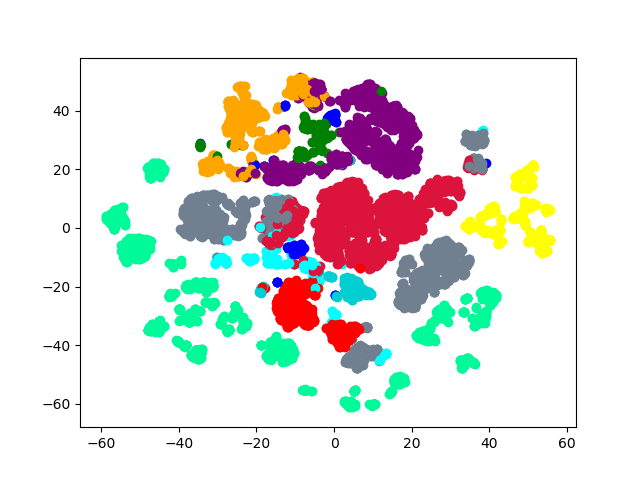
\includegraphics[width=0.8\linewidth]{media/cluster_1.png}
    \caption{KMeans聚类结果}\label{fig:kmeans}
\end{figure}
\subsubsection{GMM(混合高斯模型)聚类分析}
\begin{figure}[hbt]
    \centering
    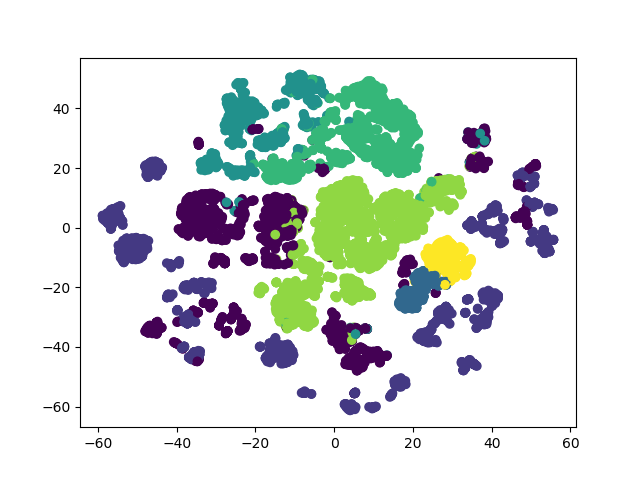
\includegraphics[width=0.8\linewidth]{media/GMM.png}    
    \caption{GMM聚类结果}\label{fig:gmm}
\end{figure}
\subsection{分类分析}
\subsubsection{朴素贝叶斯}
\paragraph{原理}
由于使用的数据每一维特征都是连续型的数据,所以其处理与离散型的朴素贝叶斯处理有所不同。\textbf{因此,假设数据的每一维都符合高斯分布,而高斯分布的均值和方差均通过训练数据中的均值和方差来代替。}
数据第$i$维取值为$x_i$的类条件概率为:
$$
    P(X_i = x_i | Y = y_j) = \dfrac{1}{\sqrt{2\pi\sigma_{ij}^2}}e^{-\frac{(x_i - \mu_{ij})^2}{2\sigma_{ij}^2}}
$$
其中$y_j$为第$j$类,$\sigma_{ij}, \mu_{ij}$分别为第$j$类第$i$维样本数据的均值和方差。具体实现时,利用了两类不同的Mapper和Reducer,其中第一对Mapper和Reducer主要用来计算训练数据中类别的先验;而第二对Mapper和Reducer用于处理计算后验并确定每一个样本所属的类别。

\paragraph{第一类Mapper}
\begin{itemize}
    \item 输入:训练数据
    \item 输出:\texttt{(label\_$k$, $v_k$)},其中label为该样本中标记的类别编号,$k$为属性的第k维,$v_k$为该样本第k维属性的取值。
\end{itemize}
\paragraph{第一类Reducer}
\begin{itemize}
    \item 输入:\texttt{(label\_$k$, [$v_{k0}, v_{k1}, \dots$])}
    \item 输出:\texttt{(label\_$k$, $mean_k$ + $\backslash t$ + $var_k$)},即计算出属于\texttt{label}类的第$k$维训练数据的均值和方差,另加法为字符串的连接。
\end{itemize}
\paragraph{第二类Mapper}
\begin{itemize}
    \item 输入:测试数据
    \item 输出:\texttt{(compute\_label, label)},其中\texttt{compute\_label}为朴素贝叶斯得到的类别编号,而\texttt{label}为数据中原本标注的类别编号。
\end{itemize}
\paragraph{第二类Reducer}
\begin{itemize}
    \item 输入:\texttt{(compute\_label, [label$_0$, label$_1$, $\dots$])}
    \item 输出:\texttt{(compute\_label, correct + $\backslash t$ + wrong)},其中\texttt{correct}为正确分类样本数目,\texttt{wrong}为错误分类数目。
\end{itemize}


\subsubsection{逻辑回归}
\section{实验心得}
可以分享您在实验环境搭建、程序编写和调试以及结果分析过程中遇到的问题和解决方法。
\appendix

% \section{源代码}
\section{参考文献}
\begin{thebibliography}{20}
    \bibitem{kmeans-mr-k} \href{http://curtis.ml.cmu.edu/w/courses/index.php/Syllabus_for_Machine_Learning_with_Large_Datasets_10-605_in_Spring_2014}{K-Means Clustering on MapReduce, CMU 10-605 2014 Spring.}
\end{thebibliography}
% \bibitem{employee_name} 中国最常见名字前50名, \texttt{https://www.sohu.com/a/164406113\_367620}
% \bibitem{employee_id} 身份证号在线生成器, \texttt{https://www.tinysoft.org/}

\end{document}
